\begin{figure}[h]
    \centering
    \begin{subfigure}[b]{\textwidth}
        \centering
        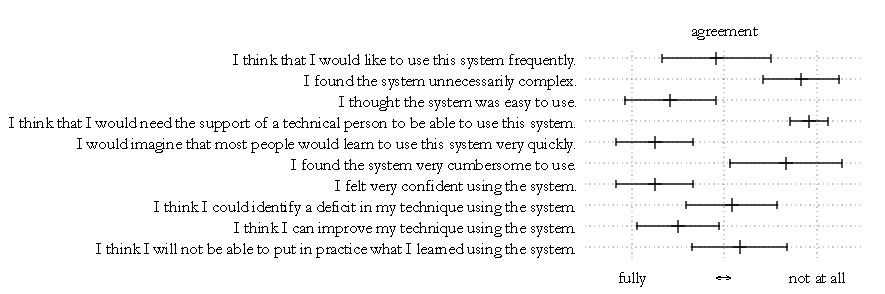
\includegraphics[width=\textwidth]{figures/plots/sus-glasses.pdf}
        \caption{First condition, the smart glasses. 6 Participants}
        \label{fig:sus-glasses}    
    \end{subfigure}
    \begin{subfigure}[b]{\textwidth}
        \centering
        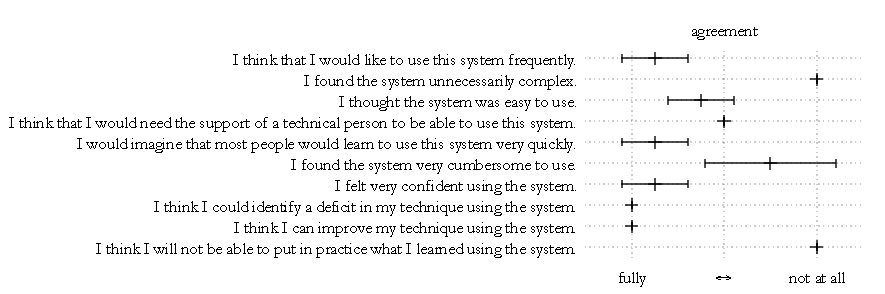
\includegraphics[width=\textwidth]{figures/plots/sus-mvn.pdf}
        \caption{Second condition, the motion tracking suit. 2 Participants}
        \label{fig:sus-mvn}
    \end{subfigure}
    \caption{SUS questions and results. A higher color saturation means more answers.}
    \label{fig:sus-results}
\end{figure}
